\chapter{The \texttt{pychoacoustics} Engine}


\section{Sound Output}
\label{sec:sound_output}

\subsubsection{Sound Output on Linux}
On Linux systems \texttt{pychoacoustics} can either output sound (numpy arrays) directly to the soundcard, or
write a wav file for each sound and call an external command to play it. Currently, support for sending
sounds directly to the soundcard is possible only through the 
\href{http://pyalsaaudio.sourceforge.net/}{alsaaudio} python module.
This module is optional, and you need to install it yourself to be able to use it.

Once it is installed, it will be detected automatically and you will be able to 
select it as the ``Play Command'' in the sound preferences dialog. When you select
"alsaaudio" as the play command, if you have multiple soundcards, you can select the 
device to which the sound will be sent. There will be also an option to set the size
of the buffer that alsaaudio uses to play sounds. If the buffer is not filled completely
by a sound (buffer size greater than number of samples in the sound), it will be zero
padded. This may lead to some latency between the offset of a sound and the onset of the
following one. If you set a value smaller than one the buffer size will be automatically 
set to the number of samples in the sound that is being played.


Using an external command to play sounds generally works very well and is fast on modern hardware.
\texttt{pychoacoustics} tries to detect available play commands on your system each time it starts up.
On Linux systems, the recommended play command is \texttt{aplay}, which is installed by default on most Linux
distributions. \texttt{aplay} supports 24-bit output on 24-bit soundcards with appropriate Linux drivers.
Other possible play commands are \texttt{play}, which is provided by \href{http://sox.sourceforge.net/}{sox} and \texttt{sndfile-play}, which
is provided by the \href{http://www.mega-nerd.com/libsndfile/}{libsndfile} tools. You can call another program by choosing ``custom'' in the
``Play Command'' drop-down menu and spelling out the name of the command in the box below.

\subsubsection{Sound Output on Windows}
Currently, on Windows systems \texttt{pychoacoustics} cannot output sounds directly to the soundcard.
It writes instead a wav file and calls an external play commands to output the sound. The recommended 
play command is \texttt{winsound}. This command supports only 16-bit
output. 

Other possible play commands are \texttt{play}, which is provided by \href{http://sox.sourceforge.net/}{sox} 
and \texttt{sndfile-play}, which is provided by the \href{http://www.mega-nerd.com/libsndfile/}{libsndfile} tools. These programs need 
to be installed by the user. If they are in the system path, \texttt{pychoacoustics} will detect them automatically. 
I am not aware of any freely available play command that can output 24-bit sound in Windows. 
Portaudio could be a used, and the Python bindings provided by pyaudio have been recently ported to Python 3. 
I have not tried this solution (and don't have much time to do it), if you want to try it, you need to be aware that in order to get 24-bit audio, 
portaudio should be probably compiled with ASIO support, and compiling portaudio on Windows with ASIO support is quite a complicated process.
Note that external media players with a graphical user interface (like foobar2000) may not work well
with \texttt{pychoacoustics}. 


\section{Parameters Files}
\label{sec:parameters_files}
Parameters files are plain text files, that can be modified through \texttt{pychoacoustics} or through a text editor. They contain a header with information that applies to all all the experimental blocks stored in a parameters file, and sections corresponding to the parameters that are specific to each experimental block store in a parameters file.
The header contains the following fields:
\begin{itemize}
\item Phones
\item Shuffle Mode
\item Sample Rate
\item Bits
\item Experiment Label
\item End Command
\end{itemize}
You can refer to Section~\ref{sec:gui_left_panel} to know what each of these fields represents.

The sections that contain the parameters for each experimental block are subdivided into fields that are separated by one or more dots. You should not change this formatting when modifying parameters files.

A fragment from a parameters file is shown below:
\begin{verbatim}
Paradigm: Adaptive
Intervals: 2 :False
Alternatives: 2 :False
\end{verbatim}
each entry here has two or three elements separated by colons. The first element represents the variable of interest, the second element its value, and the third element is a logical value that determines whether the \texttt{inSummary} checkbox will be checked or not (see Section \ref{sec:tabular_results_files} for more info on this). You can have one or more spaces between each element and the colon separator. Each entry has to be written on a single line.

\section{Results Files}
\label{sec:results_files}
\texttt{pychoacoustics} outputs several types of results files. If you name your results file ``myres'', the following files will be output:
\begin{itemize}
\item \verb+myres.txt+, ``block summary''
\item \verb+myres_full.txt+ ``full file''
\item \verb+myres_table.csv+ ``table block summary''
\end{itemize}
two further files can be derived from these:
\begin{itemize}
\item \verb+myres_res.txt+ ``session summary''
\item \verb+myres_table_processed.txt+ ``table session summary''
\end{itemize}
The ``block summary'' results file has no special suffix, and contains summaries for each experimental 
block that was run. The ``full'' results file has a ``\_full'' suffix and contains information 
for each single trial. The ``block summary'' results file can be usually processed to obtain 
a ``session summary'' results file with a ``\_res'' suffix, that contains summaries for an 
entire experimental session. In this file the results are averaged across different blocks 
that have exactly the same parameters. 

All these files are human and machine-readable, but they are not very machine-friendly 
for data analysis. That is, they can require quite a lot of either manual 
work or programming code to separate the headers and the labels from the 
values of interest (e.g., thresholds or \emph{d'} values) before the data can be 
input to a statistical software package. For this reason, \texttt{pychoacoustics} 
outputs also a ``block summary table'' result file with a ``\_table'' 
suffix that is written in a tabular format, and contains summaries for 
each experimental block that was run. This file can be further processed 
to obtain a ``session summary table'' results file with a ``\_table\_processed'' 
suffix, that contains summaries for an entire experimental session. In this file 
the results are averaged across different blocks that have exactly the same 
parameters stored in the ``\_table'' file.

In order to obtain the ``\_res'' and ``\_table\_processed'' session summary files you need to use the 
appropriate functions that can be accessed from the ``File'' menu. Alternatively, you can check the 
``Process results when finished'' checkbox in the ``Preferences'' window to let \texttt{pychoacoustics} 
automatically process these files at the end of an experimental session. If processing the result files 
manually, choose ``Process Results'' from the ``File'' menu, to convert a block summary file into 
a ``\_res'' session summary file. Choose ``Process Results Table'' to convert a block summary table 
file into a ``\_table\_processed'' session summary file. In both cases you will need to use the appropriate 
subfunction for the paradigm (e.g., adaptive, constant 1-interval 2-alternatives, etc\ldots) that was 
used in the experiment. You can choose to process all blocks present in the file (default action), the 
last $n$ blocks (of each condition), or a range of blocks (for each condition). Once you have selected 
the file to process and specified the blocks to process you can click ``Run!'' to perform the processing.

The tabular results files are comma separated value (csv) text files that can be opened in a text file 
editor or a spreadsheet application. The separator used by default is the semicolon ``;'', 
but another separator can be specified in the \texttt{pychoacoustics} preferences window. 
When processing block summary table files, make sure that the csv separator in the 
``Process Results Table'' window matches the separator used in the file.

\subsubsection{Tabular Results Files}
\label{sec:tabular_results_files}
The tabular result files contain a number of default columns, that are 
specific to the paradigm used in the experiment (e.g., threshold, number of trials etc\ldots). 
Columns with additional parameters can be stored in these files. Several text fields and 
choosers in \texttt{pychoacoustics} have what we will call \texttt{inSummary} check boxes. 
Some of these are shown marked by ellipses in Figure~\ref{fig:inSummaryCheckBoxes}.
 \begin{figure}[!h]
   \caption{\texttt{inSummary} check boxes.}
   \centering
   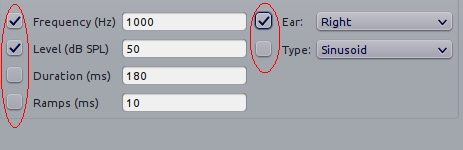
\includegraphics{Figures/inSummaryCheckBoxes.png}
   \label{fig:inSummaryCheckBoxes}
 \end{figure}
 In the example shown in Figure~\ref{fig:inSummaryCheckBoxes} the frequency, level and ear 
parameters will be stored, each in a separate column, in the block summary table (``\_table'') 
file, while the parameters corresponding to the unchecked boxes (duration, ramps and type) will be not. 
This is useful if you are running an experiment in which you are systematically 
varying only a few parameters across different blocks, and want to keep track of 
only those parameters. The \texttt{inSummary} check boxes also provide visual 
landmarks for quickly spotting the widgets with your parameters of interest in \texttt{pychoacoustics}.

Notice that the ``Process Results Table'' function, as mentioned in the previous 
section, will average the results for blocks with the same parameters 
stored in the block summary table (``\_table'') file.
This means that if you are varying a certain parameter (e.g., level) 
across blocks, but you don't check the corresponding \texttt{inSummary} check box (for each block), the value
of the parameter will not be stored in the block summary table (``\_table'') file, 
and as a consequence the ``Process Results Table'' function will not be able 
to sort the blocks according to the ``level'' parameter, and will average the 
results across all blocks. Not all is lost, because the ``level'' parameter will be nonetheless stored in the
``block summary'' file, but you will need more work before you can process your results with a statistical software package.

\subsubsection{Log Results Files}
\texttt{pychoacoustics} automatically saves backup copies of the ``block summary'' and ``full'' files in a backup folder. 
On Linux systems this folder is located in 
\begin{verbatim}
~/.local/share/data/pychoacoustics/data_backup
\end{verbatim}
on Windows systems it is located in
\begin{verbatim}
C:\\Users\username\.local\share\data\pychoacoustics\data_backup
\end{verbatim}
where \texttt{username} is your account login name.
A separate file is saved for each block of trials that is run. These files are named according to
the date and time at which the blocks were started (the naming follows the YY-MM-DD-HH-MM-SS scheme). 
Unlike other results files, that are written only once a block of trials has been completed,
these log results files get written as soon as information is available (e.g., a new line
in the ``full'' results file is written at the end of each trial).

\subsubsection{Adaptive and Weighted Up/Down Result Files}
\subsubsection{Adaptive and Weighted Up/Down Interleaved Result Files}
\subsection{Constant m-Intervals n-Alternatives Result Files}
\subsection{Multiple Constants m-Intervals n-Alternatives Result Files}
\subsection{Constant 1-Intervals 2-Alternatives Result Files}
\subsection{Multiple Constants 1-Intervals 2-Alternatives Result Files}
\subsection{Constant 1-Pair Same/Different Result Files}
\section{Block Presentation Position}
\label{sec:shuffling}

%The presentation of the blocks during an experimental session can be randomized,
%while the order in which the blocks are stored in a parameters file remains invariant. 
We will define the serial position at which a block is presented
during an experimental session as its ``presentation position'', and the serial
position at which a block is stored in a parameters file as its ``storage point''.

Clicking the ``Shuffle'' button randomises the presentation positions of the blocks, but leaves
the order in which the blocks are stored in a parameters file untouched. The ``Previous'' and ``Next'' buttons,
as well as the ``Jump to Block'' chooser let you navigate across the blocks storage points, while the 
``Previous Position'', and the ``Next Position'' buttons,
as well as the ``Jump to Position'' chooser let you navigate across the blocks presentation
positions. 

The block presentation positions are recorded in the parameters files. This is useful in case you have 
to interrupt an experimental session whose block presentation positions had been randomized, before it is finished, and continue it at a later date.
In this case you can save the parameters file, reload it next time, and let the listener complete the experimental blocks
that s/he had not run because of the interruption. Notice that each time you load a parameters file \texttt{pychoacoustics} will automatically
move to the first block presentation position. Therefore, you will have to note down what was the last block that your listener had run in the interrupted 
session (or find out by looking at the results file) and move to the presentation position of the following block yourself.

By default clicking on the ``Shuffle'' button performs a simple full randomization of the block presentation positions.
However, you can specify more complex shuffling schemes in the ``Shuffling Scheme'' text field. Let's say you want to
present two tasks in your experiment, a frequency discrimination and an intensity discrimination task. Each task
has four subconditions, (e.g.\ four different base frequencies for the frequency discrimination task and four
different base intensities for the intensity discrimination task). Your parameters file will contain eight blocks in total,
blocks one to four are for the frequency discrimination task and blocks five to eight are for the intensity discrimination task.
During the experiment you want your participants to run first the four frequency discrimination conditions in random order, and afterwards the
four intensity discrimination conditions in random order. To achieve this you can enter the following shuffling scheme:
\begin{verbatim}
([1,2,3,4], [5,6,7,8])
\end{verbatim}
basically you specify sequences (which can be nested) with your experimental blocks, sequences within round parentheses \texttt{()} are
not shuffled, while sequences within square brackets \texttt{[]} are shuffled. Following the previous example, if you want to present
first the four blocks of one of the tasks (either frequency or intensity) in random order, and then the four blocks of the other task
in random order, you would specify your shuffling scheme as follows:
\begin{verbatim}
[[1,2,3,4], [5,6,7,8]]
\end{verbatim}
on the other hand, if you want to present first the four blocks of one of the tasks (either frequency or intensity)
in sequential order and then the four blocks of the other task in sequential order, you would specify your shuffling scheme
as follows:
\begin{verbatim}
[(1,2,3,4), (5,6,7,8)]
\end{verbatim}
you can have any variation you like on the theme, and the lists can be nested ad libitum, so for example
you could have:
\begin{verbatim}
[(1,2,[3,4]), (5,6,7,8)]
\end{verbatim}
this would instruct \texttt{pychoacoustics} to present first either the four frequency conditions
or the four intensity conditions. The first two frequency conditions are presented sequentially,
while the last two are shuffled. To save typing you can give ranges rather than listing all blocks individually.
For example:
\begin{verbatim}
([1-4], [5-8])
\end{verbatim}
is equivalent to:
\begin{verbatim}
([1,2,3,4], [5,6,7,8])
\end{verbatim}






\section{OS Commands}
\label{sec:end_cmd}

\texttt{pychoacoustics} can be instructed to run operating system (OS) commands
at the end of an experiment. This may be useful to run custom scripts that may
analyse the result files, backup result files or perform other operations. 

In the control window, you can enter commands that you want to be executed at the
end of a specific experiment in the "End Command" box. This command will be saved
in the parameters file of the experiment.

In the "Preferences Dialog", under the "Notifications" tab you can instead set a command
that will be executed at the end of each experiment you run, or $n$ blocks before the end of each experiment you run. 
These commands should be entered in the "Execute custom command" boxes.

The commands that you can execute are OS commands, therefore they are different on Linux
and Windows platforms. On Linux, for example, assuming that you store all your experimental
results in the directory "/home/foo/exp/", you could automatically make a backup of these
files in the directory "/home/foo/backup/exp/" by using the command
\begin{verbatim}
rsync -r -t -v --progress -s /home/foo/exp/ /home/foo/backup/exp/
\end{verbatim}

To make things more interesting, you can use some special strings to pass \texttt{pychoacoustics}
internal variables to your commands. For example, if you want to copy the results file of
the current experiment to the directory "/home/foo/res/", you can use the command
\begin{verbatim}
cp [resFile] /home/foo/backup/exp/
\end{verbatim}
here the special string \verb+[resFile]+ will be converted to the name of the file where \texttt{pychoacoustics}
has saved the data. A full listing of these special strings is given in Table~\ref{tab:end_cmd}.

\begin{table}[htbp]
\caption{Special strings for OS end command.} 
\begin{tabular}{ll}
\toprule

\textbf{String} & \textbf{Variable}  \\
%"[resDir]", "[resFile]",        "[resFileFull]", "[resFileRes]", "[resTable]", "[listener]", "[experimenter]"
\midrule
\verb+[resDir]+ & Results file directory \\
\verb+[resFile]+ & Block summary results file \\
\verb+[resFileFull]+ & Full results file \\
\verb+[resFileRes]+ & Session summary results file \\
\verb+[resTable]+ & Block summary table results file \\
\verb+[listener]+  & Listener label \\
\verb+[experimenter]+  & Experimenter ID \\

\bottomrule
\end{tabular}
\label{tab:end_cmd}
\end{table}

\section{Preferences Settings}
\label{sec:preferences}
All the settings that can be manipulated in the ``Preferences'' dialog, as 
well as the ``Phones'' and ``Experimenters'' dialogs are stored in a file 
in the user home directory. On Linux this file is located in:
\begin{verbatim}
~/.config/pychoacoustics/preferences.py
\end{verbatim}
On Windows, assuming the root drive is ``C'' it is located in:
\begin{verbatim}
C:\\Users\username\.config/pychoacoustics\preferences.py
\end{verbatim}
where \verb+username+ is your Windows login username.
Although I strive to avoid this, the way in which the preferences settings are stored 
may change in newer versions of pychoacoustics. This means that when pychoacoustics is 
upgraded to a newer version it may sometimes not start or throw out errors. To address 
these issues, please, try removing the old preferences file. Of course this means that 
you're going to lose all the settings that you had previously saved. To avoid loosing 
any precious information, such as the calibration values of your headphones, write down 
all important info before removing the preferences file.


\section{Response Mode}
\label{sec:response_mode}

\texttt{pychoacoustics} was designed to run interactive experiments in which a listener
hears some stimuli and gives a response through a button or key press. This is the default
mode, called ``Real Listener'' mode. \texttt{pychoacoustics} provides two additional response
modes, ``Automatic'' and ``Simulated Listener''. These modes can be set through the control window.

In ``Automatic'' response mode, rather than waiting for the listener to give a response,
\texttt{pychoacoustics} gives itself a response and proceeds to the next trial. The probability
that this automatic response is correct can also be set through the control window.
The ``Automatic'' response mode has two main functions. The first is testing and debugging
an experiment. Rather than running the experiment yourself, you can launch \texttt{pychoacoustics}
in ``Automatic'' response mode and check that everything runs smoothly, the program doesn't crash,
and the result files are saved correctly. The second function of the automatic response mode is to allow
passive presentation of the stimuli. Some neuroimaging experiments (e.g.\ electroencephalographic or
functional magnetic resonance recordings) are performed with listeners passively listening to the stimuli.
These experiments usually also require that the program presenting the stimuli sends triggers to the
recording equipment to flag the start of a trial. Potentially this can also be done in \texttt{pychoacoustics}
(and we've done it in our lab for electroencephalographic recordings), but at the moment this functionality
is not implemented in a general way in the program.

The ``Simulated Listener'' mode is simply a hook that allows you to redirect the control flow of the program 
to some code that simulates a listener and provides a response. Notice that \texttt{pychoacoustics} does not
provide any simulation code in itself, the simulation code has to be written by you for a specific experiment.
If no simulation code is written in the experiment file, \texttt{pychoacoustics} will do nothing in simulated
listenr mode. Further details on how to use the ``Simulated Listener'' mode are provided in Section~\ref{sec:simulations}.

Both the ``Automatic'' and the ``Simulated Listener'' make recursive function calls. In Python the number of recursive function
calls that you can make is limited. If your experiment passes this limit \texttt{pychoacoustics} will crash. The limit can be
raised, up to a certain extent (which is dependent on your operating system, see the documentation for the setrecursionlimit function in the Python \texttt{sys} module) through the ``Max Recursion Depth'' setting that you can
find in the preferences window, or set through a command line option when running \texttt{pychoacoustics} from the command line.
Notice that the total number of recursive calls that your program will make to complete an experiments will be higher than the number of
trials in the experiment, so you should set the ``Max Recursion Depth'' to a value higher than the number of trials you're planning
to perform (how much higher I don't know, you should find out by trial and error, a few hundred points higher is usually sufficient).
If you're planning to run a very high number of trials in ``Automatic'' or ``Simulated Listener'' mode, rather than raising 
the max recursion depth, it may be better to split the experiment in several parts. You can always write a script that automatically
launches \texttt{pychoacoustics} from the command line instructing it to load a given parameters file. On UNIX machines you could write a shell script to do that, 
but an easier way is perhaphs to use python itself to write the script. For example, the \texttt{python} script could be:
\begin{lstlisting}
#! /usr/bin/env python
for i in range(5):
   cmd = "pychoacoustics --file prms.prm -l L1 -s s1 -q -a \
         --recursion-depth 3000" 
\end{lstlisting}[
here we're telling \texttt{pychoacoustics} to load the parameters file \texttt{prms.prm}, set the listener identifier to ``L1'' and the session label to s1. 
The \texttt{-q} option instructs the program to exit at the end of the experiment. 
This way the recursion depth count is effectively restarted each time \texttt{pychoacoustics} is closed and launched again from the script. 
When the \verb+--recursion-depth+ option is passed as a command line argument, as in the example above, it overrides 
the max recursion depth value set in the preferences window. If the \verb+-a+ option is passed, as in the examples above, \texttt{pychoacoustics} will start
automatically at the beginning of each of the five series . This is useful for debugging or simulations, so that you can start the script and
leave the program complete unattended (you need to make sure that the ``Shuffling Mode'' is not set to ``Ask'' and that you pass listener
and session labels if you want the program to run completely unattended). 

%%% Local Variables: 
%%% mode: latex
%%% TeX-master: "pychoacoustics_manual"
%%% End: 

